The frontend is built using the JavaScript framework Angular 4. Other large frameworks were also considered but in the end Angular seemed like the best choice. It is used in a lot of web applications so it's easy to find tutorials, there is a lot of support for it, there are many existing packages that can be imported and it is used a lot in the industry.

The site consist of a number of components. These include the different pages in the application but also other visually large parts such as the gamification elements. There are services that keep track of information used by different components and also one that is in charge of the backend calls.

The CSS library Bootstrap was used to get a clean and consistent design. To achieve a distinct and personal look a color scheme was decided upon. For this the dark blue color of LTU was used as a base.

\subsection{Authentication}
\subsubsection{Login}
To authenticate yourself on login you are by default prompted to sign in with LTU's weblogon CAS (central authentication service). 
This provides you with a ticket as an URL parameter and redirects you to path: \url{https://frontend\_ip/Auth} which in turn contacts backend with said ticket to check its validity. If validated the backend responds with a status code of 200 OK and a JSON object containing authentication tokens for the user which are saved in local storage. In any other case the user receives status code 401 unauthorized and is prompted to login again.
\begin{figure}[hb]
    \centering
    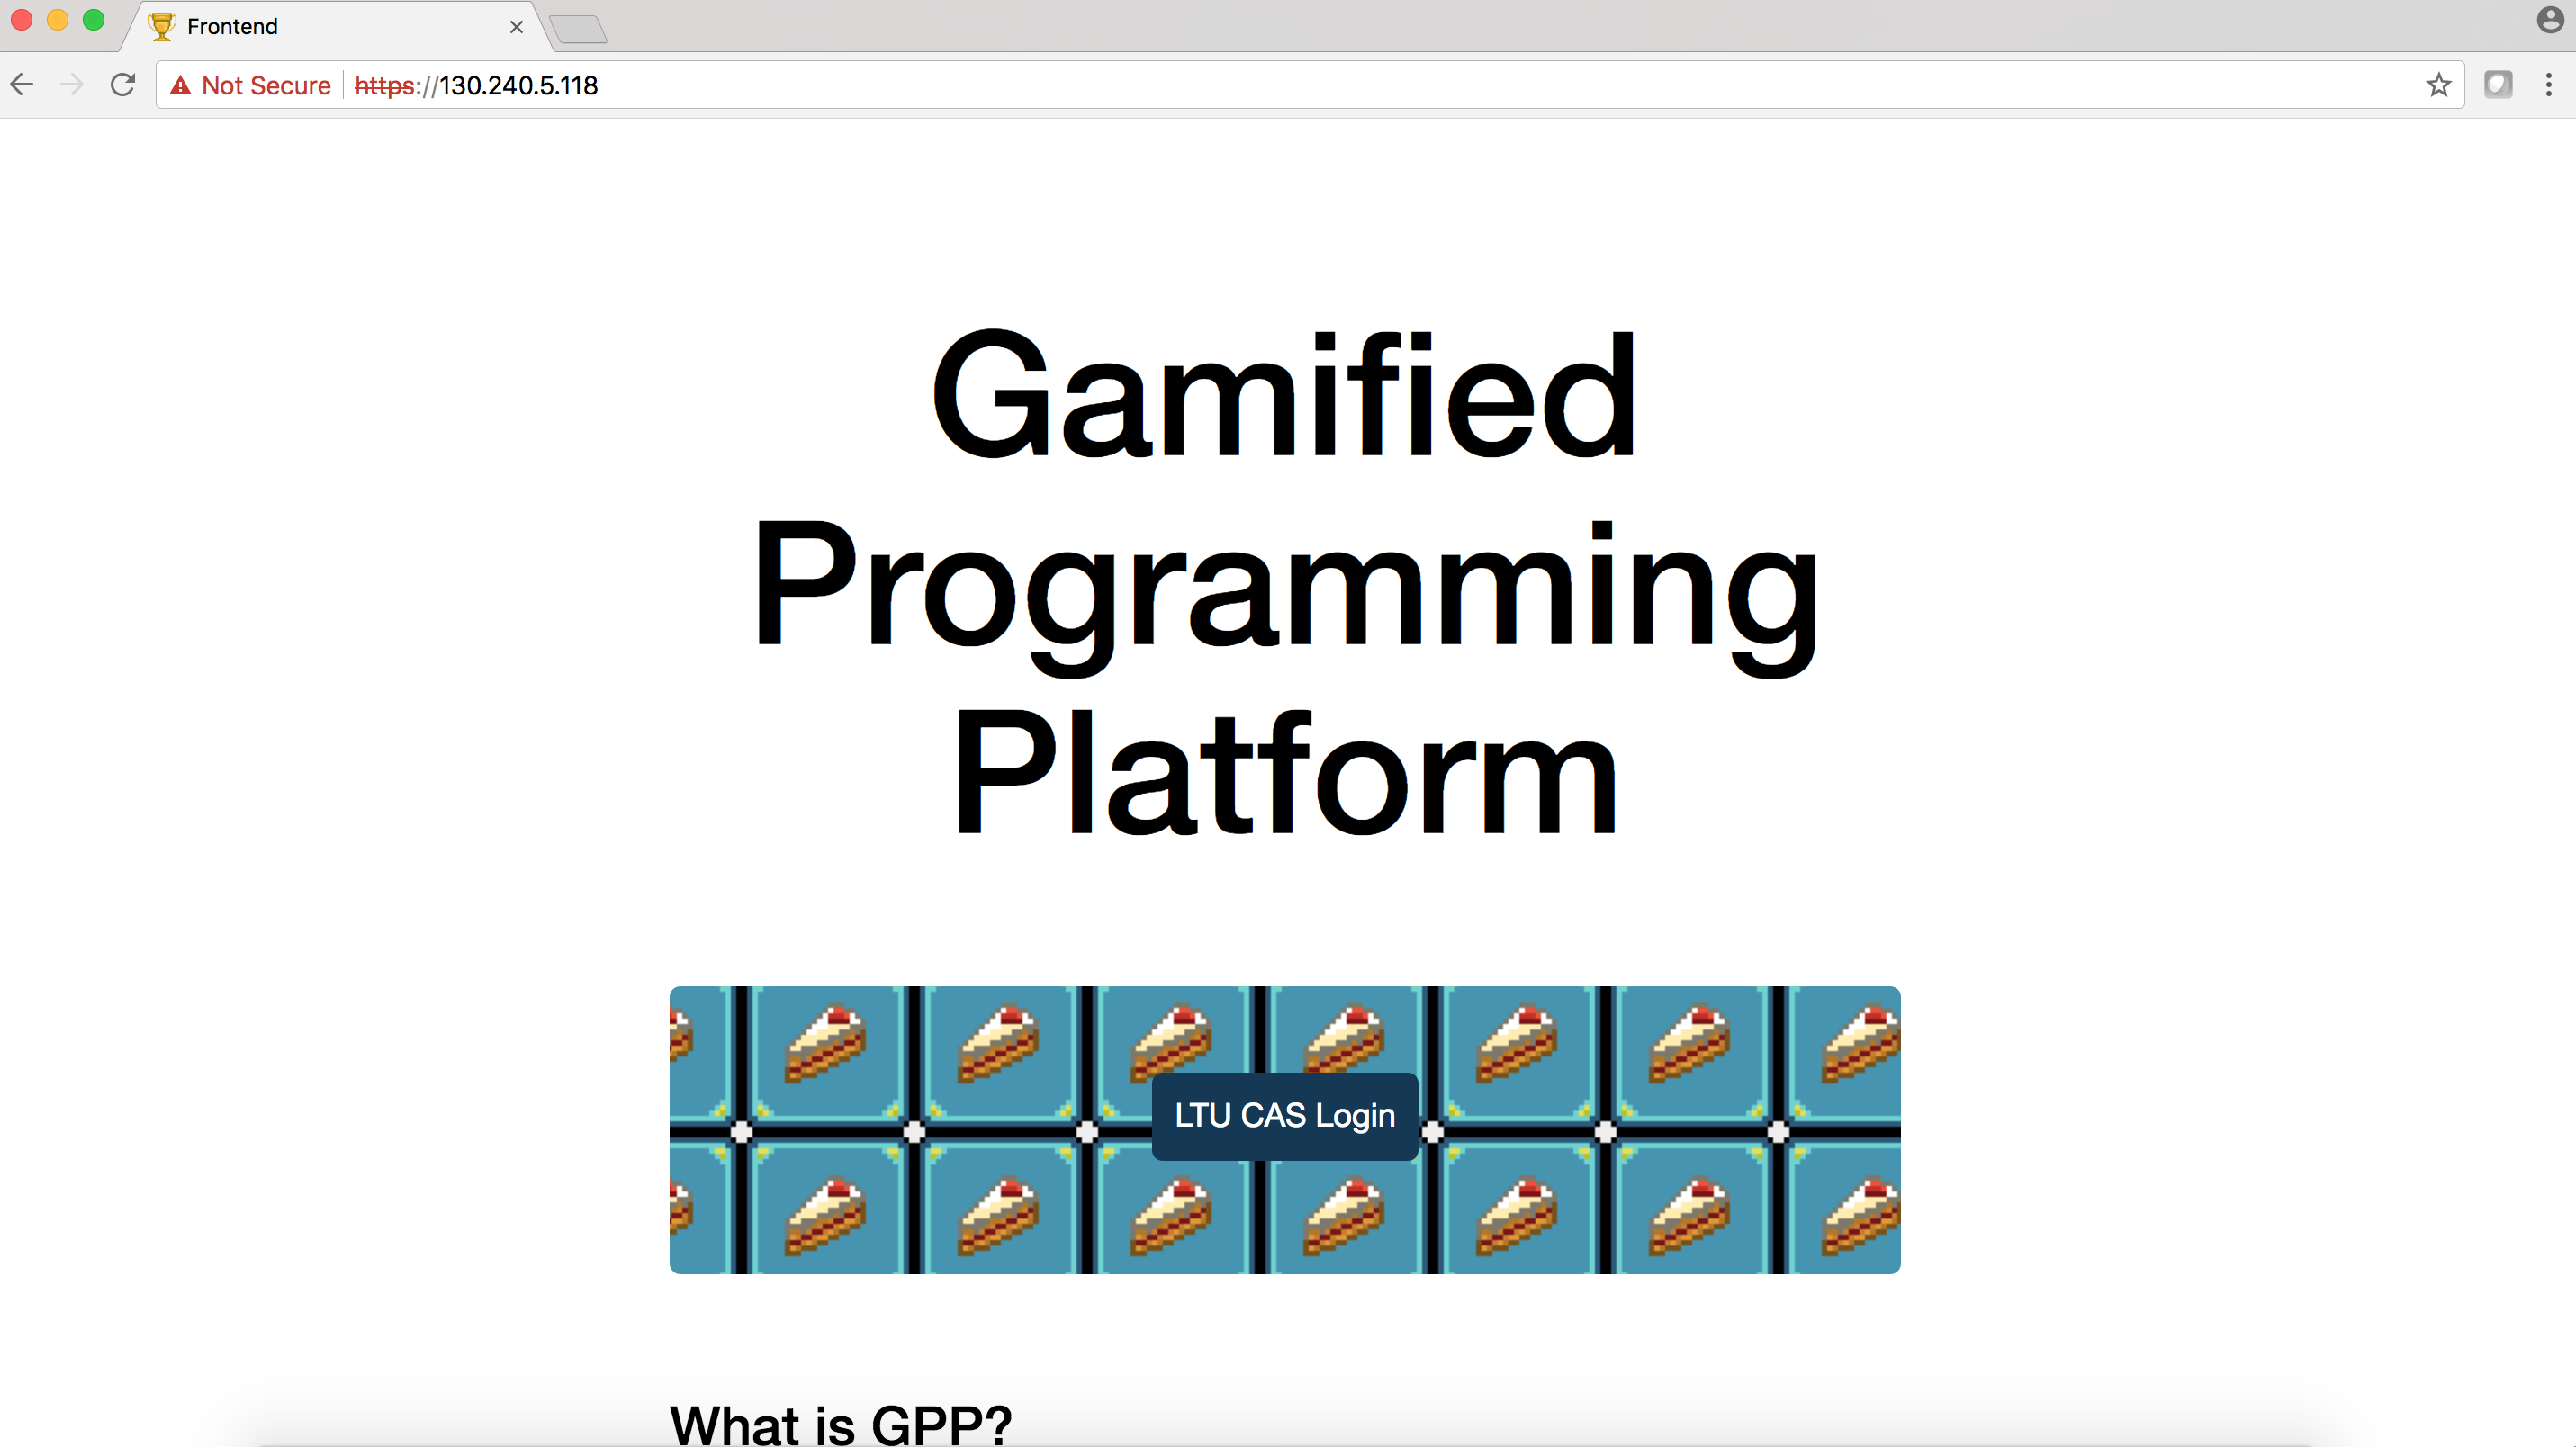
\includegraphics[width=\textwidth]{login.png}
\end{figure}

\subsubsection{Auth interceptor}
The main purpose of this interceptor is to modify all requests by setting the authentication field in the header of the request for authenticated users. More than this it collects failed requests in the case of token expiration and tries to refresh the token to retry all failed requests automatically and stay logged in without the user being aware of affected.

\subsection{User page}
Since the user page acts as the front page of the site it should display a good overview to the user. Therefore all courses that a user either has joined or created will be displayed here. To not take up too much space each course is a collapsed panel that can be opened to show any gamification elements available in the course. By clicking on the name of the course the user will be redirected to the the page for that course.

It is also possible to join a course by selecting a course from a list. This list is displayed in a modal opened by the button above the courses you have joined.  The list does not only show the course code or the name of the course but also the creator of the course. This is because there can be many courses with the same name and/or code.

On the right half of the page you can see which courses you have requested to join and can the requests be canceled. The courses that have allowed students to join the course directly without any confirmation from the teacher will of course not be displayed here. Below the requests there's a list showing any invites sent by teachers to the user. The invites can be accepted or declined.

\subsection{Assignment}
\subsubsection{Assignment Page}
The assignment component is used for displaying and for submitting a solution to an assignment. The component consists of three key fields. A feedback field for displaying server response from testr. A description field for showing the assignment description and finally an in-browser editor. 

The decision to implement an in-browser editor for writing the code was made early on as it was seen as more intuitive than having to write your code using your own editor and then uploading files to the site.

First iteration of the assignment component implemented an editor called CodeMirror, however this editor was dropped and replaced by an implementation of ace editor, which had far many more options in terms of customization such as size of editor and theme. Ace editor also had better support for switching between syntax highlighting of different languages, while CodeMirror required us to reload editor upon switching language. 

\subsubsection{Create Assignment}
The create assignment page is used for both creating and editing assignments. An assignment consists of a name, description, available languages and flag whether or not the syntax of the code should be tested using lint. 

The assignment description implements markdown, which is a format language for parsing text to correct HTML. This allows a teacher to add different sized headers, lists, embedded pictures, links, code blocks with syntax highlighting. Early version of the create assignment page implemented a live-preview for writing the description, however got removed to maintain consistent design with the create course page. 

The create assignment page also contains a field for creating and editing input-output tests. A teacher can add multiple tests for verifying the code against multiple inputs.

Once an assignment is ready to be submitted, an API call to backend to create new assignment will be made and if that call is successful, additional calls for adding input-output tests can be made. 

\subsection{Services}
In AngularJS, a service is a function or object that is accessible from anywhere in the application. On the frontend, services are used regularly as a means to reuse code, such as API calls to backend, as well as to maintain data across several pages. In the following sections some of the more important and well-used services are detailed.

\subsubsection{BackendService}
The BackendService is the center of all our communication with the backend. Every component or service that needs to either get or post information to or from the backend does so through this service. By requiring all calls to go through this service, we can perform all error handling in one place as well as ensuring that all calls are sent in a similar fashion. All calls expects a response with a JSON body. If there is no relevent information to send in the body an empty JSON body should be sent.

All of BackendService's functions return a Promise that will eventually resolve to the response from the backend. In the event that a request fails, a Toast containing the error message is displayed to the user. 

\subsubsection{AssignmentService and CourseService}
The AssignmentService is used to keep track of assignments belonging to a specific course. Information about assignments are stored in the service to remove the need of fetching assignments all the time when navigating the course page (e.g., going from the course page to the assignment page and back). The service is also used to keep the information up-to-date with changes that comes as a result of user action. For example, if a teacher creates a new assignment, we only fetch the new assignment from backend and adds it to the already saved list of assignments.

The CourseService fulfil the same purposes as the AssignmentService, but for courses instead of assignments as the name suggests.
